\documentclass{standalone}
\usepackage{graphicx}	
\usepackage{amssymb, amsmath, amsthm}
\usepackage{color}

\usepackage{tikz}

\definecolor{light}{RGB}{220, 188, 188}
\definecolor{mid}{RGB}{185, 124, 124}
\definecolor{dark}{RGB}{143, 39, 39}
\definecolor{highlight}{RGB}{180, 31, 180}
\definecolor{gray10}{gray}{0.1}
\definecolor{gray20}{gray}{0.2}
\definecolor{gray30}{gray}{0.3}
\definecolor{gray40}{gray}{0.4}
\definecolor{gray60}{gray}{0.6}
\definecolor{gray70}{gray}{0.7}
\definecolor{gray80}{gray}{0.8}
\definecolor{gray90}{gray}{0.9}
\definecolor{gray60}{gray}{0.95}

\begin{document}

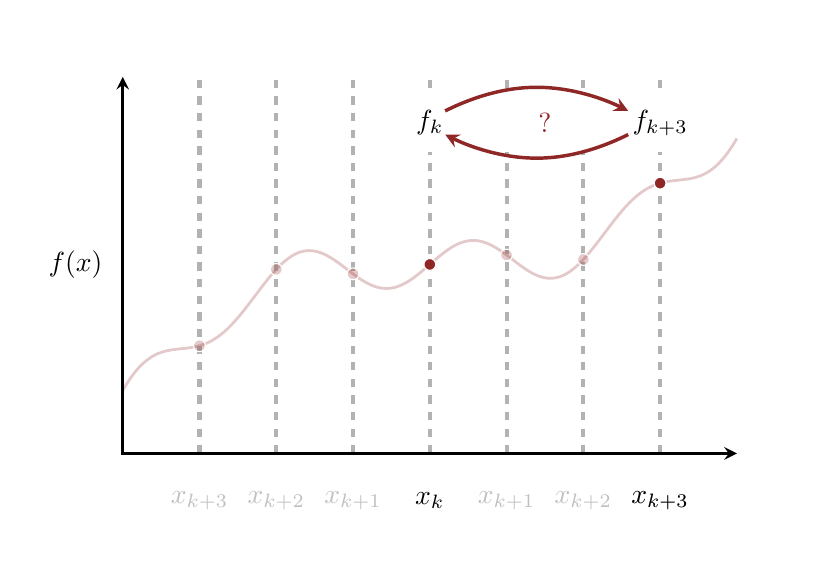
\begin{tikzpicture}[scale=0.3]
  \pgfmathsetmacro{\dx}{0}
  
  \draw[white] (-17 + \dx, -12) rectangle (15 + \dx, 10);

  \draw[domain=-13:13, smooth, samples=150, line width=1, variable=\x, color=dark, opacity=0.25] 
    plot ({\x + \dx}, {\x * \x * \x / 350 + sin(\x * 50)});

  \foreach \x [count=\i] in {-9.75, -6.5, -3.25} {
    \pgfmathsetmacro{\delta}{int(4 - \i)};
    \node[opacity=0.25] at (\x + \dx, -10) { $x_{k + \delta}$ };
  }
  
  \node[] at (0 + \dx, -10) { $x_{k}$ };
  
  \foreach \x [count=\i] in {3.25, 6.5, 9.75} {
    \pgfmathsetmacro{\delta}{int(\i)};
    \node[opacity=0.25] at (\x + \dx, -10) { $x_{k + \delta}$ };
  }
  
  \node[] at (9.75 + \dx, -10) { $x_{k + 3}$ };
  
  \foreach \x in {-9.75, -6.5, ..., 9.75} {
    \draw[dashed, color=gray70, line width=1.5] (\x + \dx, -8) -- +(0, 16);
    \fill[color=dark, opacity=0.25] (\x + \dx, {\x * \x * \x / 350 + sin(\x * 50)}) circle (0.25);
    \draw[color=white] (\x + \dx, {\x * \x * \x / 350 + sin(\x * 50)}) circle (0.25);
  }
  
  \fill[white] (-1 + \dx, 4.75) rectangle (11 + \dx, 7.25);
  \node[] at (0 + \dx, 6) { $f_{k}$ };
  \node[] at (9.75 + \dx, 6) { $f_{k + 3}$ };
  
  \begin{scope}[shift={(-0.35, 0)}]
    \draw[->, >=stealth, line width=1.25, dark] (1, 6.5) 
                                               .. controls (2, 7) and (3.375, 7.5) 
                                               .. (4.875, 7.5) 
                                               .. controls (6.375, 7.5) and (7.75, 7) 
                                               .. (8.75, 6.5);
    \draw[<-, >=stealth, line width=1.25, dark] (1, 5.5) 
                                               .. controls (2, 5) and (3.375, 4.5) 
                                               .. (4.875, 4.5) 
                                               .. controls (6.375, 4.5) and (7.75, 5) 
                                               .. (8.75, 5.5);
  \end{scope}
 
  \node[dark] at (4.875 + \dx, 6) { $?$ };
  
  \foreach \x in {0, 9.75} {
    \fill[color=dark] (\x + \dx, {\x * \x * \x / 350 + sin(\x * 50)}) circle (0.25);
    \draw[color=white] (\x + \dx, {\x * \x * \x / 350 + sin(\x * 50)}) circle (0.25);
  }

  \draw [->, >=stealth, line width=1] (-13 + \dx, -8) -- +(26, 0);
  \draw [->, >=stealth, line width=1] (-13 + \dx, -8.058) -- +(0, 16);
  \node[text=black] at (-15 + \dx, 0) { $f(x)$ };
  
\end{tikzpicture}

\end{document}  